\documentclass{article}
\usepackage[utf8]{inputenc}
\usepackage{url}
\usepackage[margin=0.75in]{geometry}
\usepackage{float}
\usepackage{graphicx}

\setlength{\parskip}{0.7em}
\setlength{\parindent}{0em}

\begin{document}
	\begin{center}
    
    	% MAKE SURE YOU TAKE OUT THE SQUARE BRACKETS
		\LARGE{\textbf{CSE 6730, Group 37 Final Report}} \\
        \vspace{1em}
        \Large{Discrete Event Simulation} \\
     
	\end{center}
    \begin{normalsize}
    
    	\section{Project Title}
        
Simulation of the Spread of Syphilis within Group Housing for the Elderly
      
		\section{Team Members}
        
      \begin{enumerate}
      	\item Aiswarya Bhagavatula (GTID 903540374)
      	\item D. Aaron Hillegass (GTID 901988533)
      	\item Siawpeng Er (GTID 903413430)
      	\item Xiaotong Mu (GTID 903529807)
      \end{enumerate}
        
	   	\section{Problem Description and Purpose}
        
    More and more communities of the elderly are suffering from outbreaks of sexually transmitted infections \cite{mcdaniel_2017}. According to Athena Health, patients over 60 account for the biggest increase of in-office treatments for sexually transmitted infections.
    
    For this study, we are going to focus on syphilis, but the methodology and resulting simulation could easily be applied to other treatable, non-deadly STIs like chlamydia and gonorrhea.
    
    There are several factors that have led to the spread of STIs among older people (especially in group housing):
    \begin{itemize}
	\item Lack of safer sex practices (such as condom use) in older individuals. People who became sexually active before AIDS are less likely to follow safe sex practices.
    \item Imbalances between the number of men and women. In retirement homes, there are typically significantly more women than men. It would not be surprising to find that the few healthy men would act as a nexus for sexually transmitted infections.
    \item Shame around testing and treatment. Older people (especially married older people) might be reluctant to tell their doctor about symptoms, get tested, and pursue treatment.
    \item Number of opportunities for transmission. In earlier times, we could expect sexual activity to diminish in the aging population.  However, with people living longer, healthier lives and the proliferation of safe erectile dysfunction drugs, people in retirement communities are more sexually active than their parents were at the same age -- especially if they live in close community with a large number of potential partners.
    \item Antibiotic resistance. Old people living in community are likely to get other kinds of bacterial infections, like strep, and take antibiotics. In the past, this was likely to wipe out undiagnosed syphilis (or chlamydia or gonorrhea) as a side-effect. As these STIs have evolved to become more antibiotic resistant, a strep-sized dose of amoxicillin is less likely to do the job.
    \end{itemize}
    
    Discrete Event Simulation (DES) was been used for long time in many healthcare simulation, ranging from health care system operation, disease progression modeling, screening modeling and health behavior modeling \cite{lebcir2017, Zhang2018}. 
    
    
     A realistic simulation of the transmission of STIs in retirement homes could be useful in deciding between different interventions.  For example, would increasing condom use by 20\% be more effective than annual STI tests?
       
     \section{Literature review}
     Propagation of Sexually transmitted diseases (STD) is modelled mainly based on the option of the social network that describes the contact between individuals. Perhaps the initial form of these models was STDSIM, created in the late 1990s and utilised in numerous HIV modelling studies \cite{10.2307/25062378}.
     
     The network models have become increasingly difficult with the use of information from the populaces under examination. One such model depicts a collection of work around demonstrating the HIV pandemic in Vancouver, which incorporates a system model of infusing drug clients and female sex laborers, with the point of evaluating the viability of various control methodologies. 
     
     To model STDs, a network model is generated with an analogy of vertices representing persons and edges representing contacts.A transmission event can happen in cases of connected edges, thus making the probability distribution of the number of edges of each node a very salient feature. Each of the edges can have various weights which directly relate to the type of interactions between the individuals. For instance, the netwrok can be modeled in three levels of interactions that determine heterosexual contact:0, no contact; 1, spousal partnership; 2, non-spousal partnership \cite{c030e9dad6134c6e9a9d18e61b852e99}.


	Although, this can be very difficult in cases with large datasets as developing models with social networks would need a large number of people to have expertise on the different fields involved like statistics, computer science, ethnography, medicine among others. 
	
	An alternative model can be built by considering mainly a few concise statistics regarding the extensive data \cite{dataset}. These contact networks make way for analysing the break of disease transmissions between persons by the use of condoms and other precautionary measures. This helps understand the impact of superspreaders as well. There are other models of STDs that are based on System Dynamics and other concepts. These are mainly aimed for making decisions on how to allocate resources to reduce STDs in a targeted testing program \cite{Kok2015}.

     \section{Data source}
    We get the data from the Centers for Disease Control and Prevention (CDC) website for parameters on syphilis. This includes:
    \begin{itemize}
    \item Rates in the general population at the ages at which people would enter retirement homes
   	\item Likelihood of transmission for different types of sexual activity (intercourse, oral, anal).
   	\item Time after infection before symptoms appear.
   	\end{itemize}
   	
   	We will also use a local retirement community to be modeled. From that administration we will find out:
   	\begin{itemize}
    \item Number of men and women 
    \item Ages at which people enter the community
    \item Duration that people stay in the community
    \item What, if any, STI testing and treatment are provided to the residents
   	\end{itemize}     
   	
   	Finally, we will do some interviews with residents to create a model of the individual:
   	\begin{itemize}
    \item Number of sexual partners per year
    \item History of STI testing and treatment 
    \item Marital status
    \item Gender
    \item Age
    \item Types of sexual activity that they engage in (if possible)
   	\end{itemize}     
   	
   	As an updated, we also successfully obtained the real data about syphilis directly from the CDC through some connections.
   	
   	\section{Methodology}
   	Our simulation will first simulate a population of people entering and exiting a single retirement community. It will use stochastic methods to give them an initial age, gender, and infection status.  It will also remove these people as move somewhere else or die. When someone dies or moves away, this creates room for a new resident.
   	
   	Within that population, we will update each individual's infection status as they become infected and get treated. We will also track if they have become symptomatic. Thus, each time an uninfected person engages in sexual activity with an infected person, we will roll the dice to decide if the uninfected person becomes infected. Each person will be symptomatic for some amount of time before seeking testing and treatment.
   	
   	We will test different interventions:
   	\begin{itemize}
    \item Increasing condom usage
    \item Periodic testing and treatment of the whole community 
    \item Promoting monogamous fluid bonding
	\item Working toward equal numbers of men and women in the community
   	\end{itemize}     
    
    \section{Modelling using Discrete Event Simulation}
	Discrete event simulation is a form of computer based modelling that provides an intuitive and flexible approach to representing complex systems. Our model simulates the dynamics of main, and casual sexual partnerships, with behavioural model parameters estimated form sexual network data.
	
	\subsection{Structural development}
	The core concepts of DES are entities, attributes, events, resources, queues, and time. In disease modeling studies, the network model will generally consist of a set of individuals connected by contacts, where it is assumed that the contacts are such that if a transmission event could take place. The use of the most important feature is how well individuals are connected. In pair-formation models developed by Dietz and Hadeler, Waldstätter, and Kretzschmar and Dietz \cite{dietz_hadeler_1988} ,the pair-formation framework allow modeling of differential infection risk among persons who are single or paired, and it has been widely used in a number of other mathematical models of sexually transmitted infections \cite{heijne_althaus_herzog_kretzschmar_low_2011, powers_ghani_miller_hoffman_pettifor_kamanga_martinson_cohen_2011,xiridou_geskus_wit_coutinho_kretzschmar_2003, ferguson_garnett_2000}.
	
	Our model include compartments that stratify the population by age, sex, partnership status, sexual risk behavior, and infection status. Transmission of sexual disease in the model occurs via unprotected sex in heterosexual partnerships (refer to Fig. \ref{fig:blockDiagram})
	
	Predictors of partnership formation varies by partnership type,risk level,, age mixing, and status-unknown partnership. In our model, there are 2 partnership statuses that are mutually exclusive. Entity can be part of the unpaired(“single”)population or paired(“married”), unpaired population can have casual partners at age-specific rates. Casual partners represent short term relationships, and they are modeled as instantaneous partnerships. Behavioral parameters were informed by the National Survey of Family Growth. Parameters and their prior distributions \cite{galer_et2019} are shown in Table \ref{tab:parameter}. 
	
	
	\begin{table}[H]
	\centering
    	\begin{tabular}{ |p{5cm}|p{7cm}|p{5cm}| } 
    		\hline
    		Parameter/Variable & Description & Distribution  \\ 
    		\hline
    		Population size & Population size for each age group & Uniformly distributed\\
    		Time step &	Time step implemented in the model & 	A day \\
			High risk & Fraction of the population defined as high risk	& 10\% (Assumption) \\
			Low risk & Fraction of the population defined as low risk & 90\% (Assumption)\\
			\hline
			\multicolumn{3}{|c|}{Testing symptomatic individuals} \\
			\hline
			Women &	Testing of symptomatic  women	& 1/(52*(0.079+0.072*Beta(4,4)))\\
			Men	& Testing of symptomatic men	& 1/(52*(0.079+0.072*Beta(4,4)))\\
			\hline
			\multicolumn{3}{|c|}{Casual partners} \\
			\hline
			High risk(HR)& Single, 65-79 HR	& Beta(3,60)\\
 						 & Single, 80-95 HR	& Beta(3,400)\\
			Low risk(LR)	 & Single, 65-79 LR	& Beta(1,160) \\
 						 & Single, 80-95 LR	&Beta(1,160)\\
 			\hline
 			\multicolumn{3}{|c|}{Among paired} \\
 			\hline
			High risk(HR)& Single, 65-79 HR	& Beta(10,70)\\
			Low risk(LR) & Single, 80-95 LR	& Beta(10,100)\\
			Treatment success(efficiency of antibiotics)	 & & Beta(190,8)\\
			\hline
			\multicolumn{3}{|c|}{Natural recovery} \\
			\hline
			Women & & 1/(52*(1.13+0.5*Beta(4,4.969)))\\
			Men & & 1/(52*(1.13+0.5*Beta(4,4.969)))\\
			Transmission probability	 & Per act probability	& Beta(5.5, 50)\\
    		\hline
    	\end{tabular}
    	\label{tab:parameter}
    	\caption{Description of parameters governing testing, natural recovery and transmission probability}
   \end{table}
   
   	we chose to fix the fraction of the population defined as high risk at constant 10\%, but accommodate uncertainty in levels of risk behavior by varying the partner change rates by relationship states and age, in each of the risk groups. Defining a set proportion of the population to belong to a risk group and varying partner change rates is a modeling convention

    

	

\begin{figure}[H]
\caption{Block Diagram of  the Simulation}
\centering
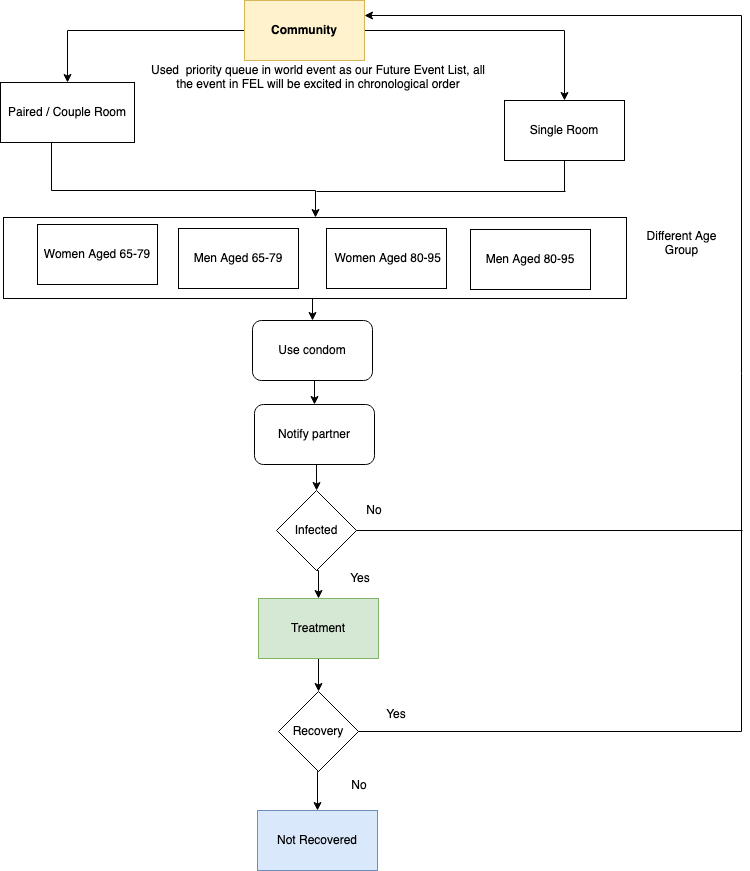
\includegraphics[width=1\textwidth]{BlockDiagram.png}
\label{fig:blockDiagram}
\end{figure}


    \section{Development Platform}
    The programming language is Python $3$. Depends on the suitability of the project, we plan to provide a Jupyter notebook for user interaction, or just a command line execution.
    
    We will use heapq as our priority queue.
    
	\subsection{Development}
	Currently, we have successfully model the World as our simulation environment. We have a set of parameters as per Table \ref{tab:parameter2}. The parameters will be updated and replaced if more suitable parameters needed.
	
	For checkpoint 1, we successfully create a simple version to have room occupied with couple or non couple. We first create the new clusters and rooms. The rooms may be occupied by couple or non couple. If more than one female and male in the room, a chance of sexual activity may occured. This resulting in the occurrence of sexually transmitted infection (STI).
	
	We shall include more working flow, especially on the intervention, treatment and prevention on our current model, so as to reflect more realistic conditions. This also serve as useful model to investigate the effect of different intervention.
	
	In the program, simply run python main.py and the result will be a list of event that occurs in the simulated environment. We shall include a complete log file with statistics in our next checkpoint. 
	     
    \begin{table}[H]
	\centering
    	\begin{tabular}{ |p{5cm}|p{7cm}| } 
    		\hline
    		Parameters & Description\\
    		\hline
    		logfile & logfile name\\
    		room\_cluster\_count & number of cluster\\
    		room\_per\_cluster\_count & number of room per cluster\\
    		prob\_new\_room\_for\_married & probability of the room as couple room\\
    		prob\_new\_single\_male & probability of a new single male\\
    		max\_age\_male\_resident & maximum age of male resident\\
    		max\_age\_female\_resident & maximum age of female resident\\
    		std\_probability & probability of having STI\\
    		mean\_age\_new\_resident & the mean age of the new resident\\ 
    		sd\_age\_new\_resident & standard deviation of the age of new resident\\
    		max\_day\_room\_empty & maximum number the room is not occupied\\
    		\hline
    	\end{tabular}
    	\label{tab:parameter2}
    	\caption{Description of parameters in the simulation}
   \end{table}

\section{Simulation result}
- we will have a table. then discussion about the result

\section{Verification and Validation}
What are the assumptions
What are the model used (cite all the paper)
Compare with the result

\subsection{Limitation of the model}
Some of the limitatio of our model:
Interaction of the factor could be more complicated .... etc (just briefly talk about it, then talk about improvement)

\section{Conclusion}
In this discrete event simulation event, we have successfully implement a simulation of the STD event in a housecare.
%	\item Aiswarya Bhagavatula (GTID 903540374)
%\item D. Aaron Hillegass (GTID 901988533)
%\item Siawpeng Er (GTID 903413430)
%\item Xiaotong Mu (GTID 903529807)

    \section{Division of Labor}
       \begin{center}
    	\begin{tabular}{ |c|c|c| } 
    		\hline
    		Task & Member  \\ 
    		\hline
    		Data collection & All \\ 
    		Programming & D.Aaron Hillegass, Siawpeng Er \\ 
    		Literature review & Xiaotong Mu, Aiswarya Bhagavatula \\ 
    		Verification / Validation of Model & Siawpeng Er, Xiaotong Mu \\
    		Final Report & All\\
    		\hline
    	\end{tabular}
    \end{center}
       
    \begin{center}
    	\begin{tabular}{ |c|c|c| } 
    		\hline
    		Task & Duration  \\ 
    		\hline
    		Data collection & 2 weeks \\ 
    		Modeling design and implementaion & 4 weeks \\ 
    		Modeling revised & 4 weeks \\ 
    		\hline
    	\end{tabular}
    \end{center}
    
    
    
    \bibliographystyle{plain}
    \bibliography{reference}
\end{normalsize}
  
\end{document}
